\section{Разработка приложений для Android}
\subsection{йцу}


\begin{frame}[fragile]
	\frametitle{Основные части приложения}

	\begin{enumerate}
	\item{\emph{AndroidManifest.xml} --- главное описание приложения, название, версия, версия SDK, список Activity, права, которые нужны приложению}
	\item{\emph{src/com.example.exampleapp/MainActivity.java} --- }
	\item{\emph{res/layout/activity\_main.xml} --- расположение элементов управления на MainActivity}
	\item{\emph{res/menu/activity\_main.xml} --- главное меню}
	\item{\emph{res/values/strings.xml} --- используемые строки (для того чтобы делать переводы на разные языки)}
	\item{\emph{gen/com.example.exampleapp/R.java} --- java файл с идентификаторами, определенными в XML файлах (чтобы использовать их в исходниках)}
	\end{enumerate}
\end{frame}

\begin{frame}[fragile]
	\frametitle{Activity}
	
	\begin{columns}[c]
	\column{2.45in}
	\emph{Activity} --- это компонент приложения, который отвечает за взаимодействие с пользователем. Обычно это окно которое заполняет весь экран (кроме строки статуса сверху), но она может также заполнять экран полностью либо быть меньше экрана.

	\medskip
	У приложения всегда есть Activity, которая появляется в момент запуска приложения, её называют "главной" (main).
	\column{2.0in}
	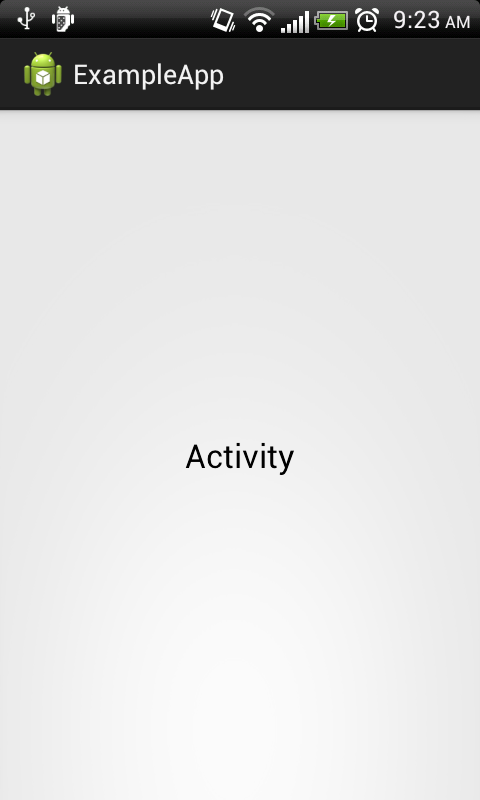
\includegraphics[scale=0.25]{2013-04-25_09-23-28.png}
	\end{columns}
\end{frame}

\begin{frame}[fragile]
	\frametitle{Как добавить Activity ?}

	\begin{enumerate}
	\item{Добавить в src/com.example.exampleapp/ java-файл с классом, унаследованным от Activity}
	\item{Добавить описание этой Activity в манифест:}
	\begin{minted}[bgcolor=bgcode,linenos=true]{bash}
	<manifest  . . .>
	    <application . . . >
	        <activity android:name=".Activity2" />
	        ...
	    </application . . . >
	    . . .
	</manifest >
	\end{minted}

	\bigskip
	Или кликнуть правой кнопкой на com.example.exampleapp и выбрать New->Other и в появивщемся окне --- Android->AndroidActivity.
	\end{enumerate}
\end{frame}


\begin{frame}[fragile]
	\frametitle{Жизненный цикл приложения}

	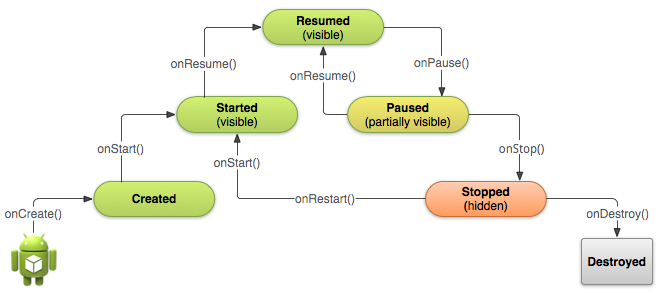
\includegraphics[scale=0.48]{basic-lifecycle.png}
\end{frame}

\begin{frame}[fragile]
	\frametitle{Как запустить новую Activity}

	\emph{Intent} --- класс для передачи данных из одной Activity в другую в момент запуска или завершения. Так что нам нужно создать объект класса Intent и вызвать метод startActivity:

	\begin{minted}[bgcolor=bgcode,linenos=true]{java}
	Intent intent = new Intent(this, Activity2.class);
	intent.putExtra(EXTRA_MESSAGE, message);
	startActivity(intent);
	\end{minted}

	\medskip
	В Activity2 message можно будет получить следущим образом:
	\begin{minted}[bgcolor=bgcode,linenos=true]{java}
	Intent intent = getIntent();
	String message = intent.getStringExtra(
	                   MainActivity.EXTRA_MESSAGE);
	\end{minted}

\end{frame}

\begin{frame}[fragile]
	\frametitle{Обработка событий}
	Первый способ --- с помощью интерфейса OnClickListener.

	\medskip
	\begin{minted}[bgcolor=bgcode,linenos=true]{java}
	protected void onCreate(Bundle savedInstanceState) {
	    /* ... */
	    Button button = (Button) findViewById(R.id.button1);
	    button.setOnClickListener(this);
	}

	public void onClick(View v) {
	    /* handle event */
	}
	\end{minted}
\end{frame}

\begin{frame}[fragile]
	\frametitle{Обработка событий}
	Второй способ --- с помощью свойства android:onClick.

	\medskip
	В файле MainActivity.xml:
	\begin{minted}[bgcolor=bgcode,linenos=true]{bash}
	<Button
	    android:id="@+id/button1"
	    ...
	    android:text="Button"
	    android:onClick="handleButton1" />
	\end{minted}

	В файле MainActivity.java надо добавить метод handleButton1:
	\begin{minted}[bgcolor=bgcode,linenos=true]{java}
	public void handleButton1(View v) {
	    /* handle event */
	}
	\end{minted}

\end{frame}

\subsection{Layouts}

\begin{frame}[fragile]
	\frametitle{Layouts}
	\begin{minted}[bgcolor=bgcode,linenos=true]{java}
	JFrame frame = new JFrame();
	JPanel panel = frame.getContentPane();

	BoxLayout l;
	l = new BoxLayout(panel, BoxLayout.Y_AXIS);
	panel.setLayout(l);

	b = new JButton("Button 1");
	panel.add(b);

	b = new JButton("B 2");
	panel.add(b);
	\end{minted}
\end{frame}



\begin{frame}[fragile]
	\frametitle{BoxLayout}
	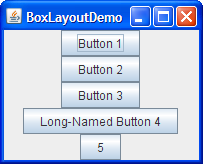
\includegraphics[scale=1]{BoxLayoutDemo.png}
\end{frame}

\begin{frame}[fragile]
	\frametitle{BorderLayout}
	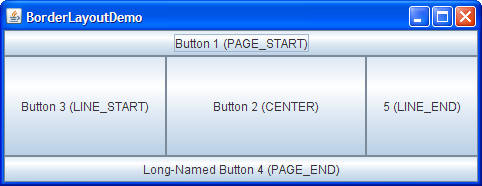
\includegraphics[scale=0.7]{BorderLayoutDemo.png}
\end{frame}

\begin{frame}[fragile]
	\frametitle{GridBagLayout}
	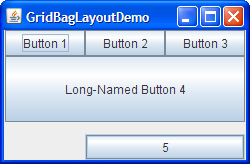
\includegraphics[scale=1]{GridBagLayoutDemo.png}
\end{frame}

\begin{frame}[fragile]
	\frametitle{GridLayout}
	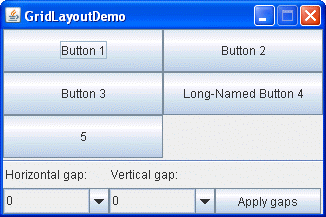
\includegraphics[scale=1]{GridLayoutDemo.png}
\end{frame}

\begin{frame}[fragile]
	\frametitle{FlowLayout}
	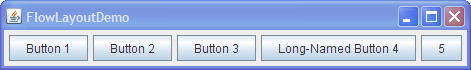
\includegraphics[scale=0.8]{FlowLayoutDemo.png}
\end{frame}

\begin{frame}[fragile]
	\frametitle{GroupLayout}
	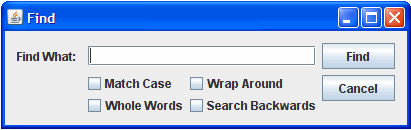
\includegraphics[scale=1]{find.png}
\end{frame}

\begin{frame}[fragile]
	\frametitle{SpringLayout}
	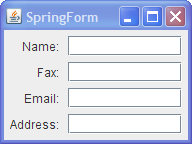
\includegraphics[scale=1]{SpringForm.png}
\end{frame}


